\documentclass[a4paper,11pt,landscape,exos]{nsi} % COMPILE WITH DRAFT
\usepackage{hyperref}

\pagestyle{empty}
\setlength{\columnseprule}{0.5pt}
\setlength{\columnsep}{1cm}
\begin{document}

\begin{multicols}{2}
\classe{\premiere spe}
\titre{
\includegraphics[width=3cm]{CAN.png} Interrogation 2}
\maketitle

\begin{enumerate}[itemsep=1em]
	\item $0{,}6\times4$
	\item Affirmation : \\
    Le point $A(-3\,;\,12)$ appartient à la parabole d'équation $y=x^2+3$ \\	$\square\;$ Vrai \qquad $\square\;$ Faux\qquad 
	\item Développer et réduire l'expression $(x-3)(2x+1)$.\\
	\item $1+\dfrac{1}{3}$ 
	\item $20\,\%$ de $70$
	\item Écriture décimale de   $\dfrac{3}{4}$ \\
	\item Multiplier une quantité par $0{,}84$ revient à la diminuer de : $\ldots\,\%$
	\item $(u_n)$ est une suite géométrique telle que $u_0=4$ et $u_1=-28$\\La raison de cette suite est :  $\ldots$
	\item Compléter par deux entiers consécutifs : \\$\ldots < \sqrt{34} < \ldots$
	\item Solution de l'équation $3x+1=8$\\
	\item Compléter.\\
      $\dfrac{18\pi}{7}=2\pi+$  $\ldots$
	\item  Factoriser   $(2x-3)^2-2(2x-3)$.\\
	%\item Dans une base orthonormée : $\vec{u}(5\,;\,-2)$ et  $\vec{v}(1\,;\,3)$.\\
    %Alors $\vec{u}\cdot\vec{v}=$ $\ldots$
	\item Déterminer l'équation réduite de la droite $(AB)$.\\    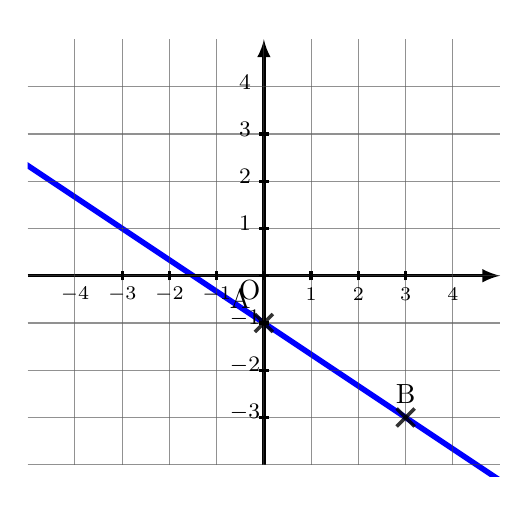
\begin{tikzpicture}[baseline,scale = 0.6]

    \tikzset{
      point/.style={
        thick,
        draw,
        cross out,
        inner sep=0pt,
        minimum width=5pt,
        minimum height=5pt,
      },
    }
    \clip (-5,-4.25) rectangle (5,5.25);
    	\draw [color={black}] (-0.3,-0.3) node[anchor = center,scale=1, rotate = 0] {O};
	\draw[color={blue},line width = 2] (-41.55,26.7)--(44.55,-30.7);
	\draw[color ={black},line width = 1.2,>=latex,->] (-5,0)--(5,0);
	\draw[color ={black},line width = 1.2,>=latex,->] (0,-4)--(0,5);
	\draw[color ={black},opacity = 0.4] (-5,1)--(5,1);
	\draw[color ={black},opacity = 0.4] (-5,-1)--(5,-1);
	\draw[color ={black},opacity = 0.4] (-5,2)--(5,2);
	\draw[color ={black},opacity = 0.4] (-5,-2)--(5,-2);
	\draw[color ={black},opacity = 0.4] (-5,3)--(5,3);
	\draw[color ={black},opacity = 0.4] (-5,-3)--(5,-3);
	\draw[color ={black},opacity = 0.4] (-5,4)--(5,4);
	\draw[color ={black},opacity = 0.4] (-5,-4)--(5,-4);
	\draw[color ={black},opacity = 0.4] (1,-4)--(1,5);
	\draw[color ={black},opacity = 0.4] (-1,-4)--(-1,5);
	\draw[color ={black},opacity = 0.4] (2,-4)--(2,5);
	\draw[color ={black},opacity = 0.4] (-2,-4)--(-2,5);
	\draw[color ={black},opacity = 0.4] (3,-4)--(3,5);
	\draw[color ={black},opacity = 0.4] (-3,-4)--(-3,5);
	\draw[color ={black},opacity = 0.4] (4,-4)--(4,5);
	\draw[color ={black},opacity = 0.4] (-4,-4)--(-4,5);
	\draw[color ={gray},opacity = 0.3] (-5,0)--(5,0);
	\draw[color ={gray},opacity = 0.3] (-5,1)--(5,1);
	\draw[color ={gray},opacity = 0.3] (-5,-1)--(5,-1);
	\draw[color ={gray},opacity = 0.3] (-5,2)--(5,2);
	\draw[color ={gray},opacity = 0.3] (-5,-2)--(5,-2);
	\draw[color ={gray},opacity = 0.3] (-5,3)--(5,3);
	\draw[color ={gray},opacity = 0.3] (-5,-3)--(5,-3);
	\draw[color ={gray},opacity = 0.3] (-5,4)--(5,4);
	\draw[color ={gray},opacity = 0.3] (-5,-4)--(5,-4);
	\draw[color ={gray},opacity = 0.3] (0,-4)--(0,5);
	\draw[color ={gray},opacity = 0.3] (1,-4)--(1,5);
	\draw[color ={gray},opacity = 0.3] (-1,-4)--(-1,5);
	\draw[color ={gray},opacity = 0.3] (2,-4)--(2,5);
	\draw[color ={gray},opacity = 0.3] (-2,-4)--(-2,5);
	\draw[color ={gray},opacity = 0.3] (3,-4)--(3,5);
	\draw[color ={gray},opacity = 0.3] (-3,-4)--(-3,5);
	\draw[color ={gray},opacity = 0.3] (4,-4)--(4,5);
	\draw[color ={gray},opacity = 0.3] (-4,-4)--(-4,5);
	\draw[color ={black},line width = 1.2] (0,-0.1)--(0,0.1);
	\draw[color ={black},line width = 1.2] (1,-0.1)--(1,0.1);
	\draw[color ={black},line width = 1.2] (-1,-0.1)--(-1,0.1);
	\draw[color ={black},line width = 1.2] (2,-0.1)--(2,0.1);
	\draw[color ={black},line width = 1.2] (-2,-0.1)--(-2,0.1);
	\draw[color ={black},line width = 1.2] (3,-0.1)--(3,0.1);
	\draw[color ={black},line width = 1.2] (-3,-0.1)--(-3,0.1);
	\draw[color ={black},line width = 1.2] (-0.1,0)--(0.1,0);
	\draw[color ={black},line width = 1.2] (-0.1,1)--(0.1,1);
	\draw[color ={black},line width = 1.2] (-0.1,-1)--(0.1,-1);
	\draw[color ={black},line width = 1.2] (-0.1,2)--(0.1,2);
	\draw[color ={black},line width = 1.2] (-0.1,-2)--(0.1,-2);
	\draw[color ={black},line width = 1.2] (-0.1,3)--(0.1,3);
	\draw[color ={black},line width = 1.2] (-0.1,-3)--(0.1,-3);
	\draw (1,-0.4) node[anchor = center, rotate=0] {\scriptsize \color{black}{$1$}};
	\draw (2,-0.4) node[anchor = center, rotate=0] {\scriptsize \color{black}{$2$}};
	\draw (3,-0.4) node[anchor = center, rotate=0] {\scriptsize \color{black}{$3$}};
	\draw (4,-0.4) node[anchor = center, rotate=0] {\scriptsize \color{black}{$4$}};
	\draw (-1,-0.4) node[anchor = center, rotate=0] {\scriptsize \color{black}{$-1$}};
	\draw (-2,-0.4) node[anchor = center, rotate=0] {\scriptsize \color{black}{$-2$}};
	\draw (-3,-0.4) node[anchor = center, rotate=0] {\scriptsize \color{black}{$-3$}};
	\draw (-4,-0.4) node[anchor = center, rotate=0] {\scriptsize \color{black}{$-4$}};
	\draw (-0.4,1.1) node[anchor = center, rotate=0] {\footnotesize \color{black}{$1$}};
	\draw (-0.4,2.1) node[anchor = center, rotate=0] {\footnotesize \color{black}{$2$}};
	\draw (-0.4,3.1) node[anchor = center, rotate=0] {\footnotesize \color{black}{$3$}};
	\draw (-0.4,4.1) node[anchor = center, rotate=0] {\footnotesize \color{black}{$4$}};
	\draw (-0.4,-0.9) node[anchor = center, rotate=0] {\footnotesize \color{black}{$-1$}};
	\draw (-0.4,-1.9) node[anchor = center, rotate=0] {\footnotesize \color{black}{$-2$}};
	\draw (-0.4,-2.9) node[anchor = center, rotate=0] {\footnotesize \color{black}{$-3$}};
	\draw[color ={black},line width = 1.25,opacity = 0.8] (2.81,-2.81)--(3.19,-3.19);\draw[color ={black},line width = 1.25,opacity = 0.8] (2.81,-3.19)--(3.19,-2.81);
	\draw[color ={black},line width = 1.25,opacity = 0.8] (-0.19,-0.81)--(0.19,-1.19);\draw[color ={black},line width = 1.25,opacity = 0.8] (-0.19,-1.19)--(0.19,-0.81);
	\draw [color={black}] (-0.5,-0.5) node[anchor = center,scale=1, rotate = 0] {A};
	\draw [color={black}] (3,-2.5) node[anchor = center,scale=1, rotate = 0] {B};

\end{tikzpicture}\\
	\item Soit la suite $(u_n)$ définie  par $u_0 = 4$ et pour $n \in \mathbb{N}$, 
    $u_{n+1} = -3u_n +4$.\\
    $u_2=$ $\ldots$
	\item $P(A\cap B)=0{,}2$\\$P(A)=0{,}3\,\,;\,\,P(B)=0{,}5$\\$A$ et $B$ sont indépendants.\\\\	$\square\;$ Vrai\qquad $\square\;$ Faux\qquad 
	\item Le discriminant du trinôme $x^2-4x+1$ est  $\ldots$
	\item Un sportif court $3\,500$ m  en $15$ min.\\
      Quelle est sa vitesse en km/h ?
	\item $f(x)=\dfrac{1}{2}x^2+8x-1$\\
    $f'(x)=$ $\ldots$
	
	%\item $q\neq 1$ \\$1+q+q^2+\ldots+q^{24}=$ \\	$\square\;$ $\dfrac{q-q^{25}}{1-q}$ \qquad $\square\;$ $\dfrac{1-q^{25}}{1-q}$\qquad 
	%\item $f(x)=-6x^2+9$\\
    %$f'(3)=$ $\ldots$
	\item Solutions de $(x-9)(x+3)  < 0$\\
	\item Soit $f\,:\,x\longmapsto (x-4)(x+10) $\\
    La représentation graphique $\mathcal{C}_f$ a pour axe de symétrie la droite d’équation :\\	$\square\;$ $x=3$\qquad $\square\;$ $x=4$\qquad $\square\;$ $x=-3$\qquad  
	
\end{enumerate}
\vfill\null
\columnbreak

\textcolor{UGLiBlue}{NOM, Prénom :\\
Date : vendredi 14/03/2025}

\end{multicols}

\newpage

\begin{multicols}{2}
    \classe{\premiere spe}
\titre{
\includegraphics[width=3cm]{CAN.png} Corrigé Interro 2}
\maketitle

\begin{enumerate}[itemsep=1em]
    \item On peut calculer ainsi : \\
        $\begin{aligned}
        0{,}6\times4&=0,1\times 6\times4\\
        &=0,1\times 24\\
        &={\color[HTML]{f15929}\boldsymbol{2{,}4}}
        \end{aligned}$
    \item Le point $A$ est sur la parabole si son ordonnée est égale à l'image de son abscisse. \\
        $\begin{aligned}
            f(-3)&=(-3)^2+3\\
            &=12
            \end{aligned}$
            \\
            Le point $A$ est bien sur la parabole.\\ L'affirmation est {\bfseries \color[HTML]{f15929}VraiE}
    \item $\begin{aligned}
          (x-3)(2x+1)&=2x^2+x-6x-3\\
          &={\color[HTML]{f15929}\boldsymbol{2x^2-5x-3}}
          \end{aligned}$\\Le terme en $x^2$ vient de $x\times 2x=2x^2$.\\Le terme en $x$ vient de la somme de $x \times 1$ et de $-3 \times 2x$.\\Le terme constant vient de $-3\times 1= -3$.
    \item $\begin{aligned}
          1+\dfrac{1}{3} &= \dfrac{1 \times 3}{3} + \dfrac{1}{3} \\
          &= \dfrac{3}{3} + \dfrac{1}{3}\\
          &  ={\color[HTML]{f15929}\boldsymbol{\dfrac{4}{3}}}
          \end{aligned}$
\vfill\null
\columnbreak  
    \item $20\,\%$ de $70 = {\color[HTML]{f15929}\boldsymbol{14}}$\\ Prendre $20\,\%$  de $70$ revient à prendre $2\times 10\,\%$  de $70$.\\
          Comme $10\,\%$  de $70$ vaut $7$ (pour prendre $10\,\%$  d'une quantité, on la divise par $10$), alors
          $20\,\%$ de $70=2\times 7=14$.
       
    \item $\dfrac{3}{4}={\color[HTML]{f15929}\boldsymbol{0{,}75}}$
    \item Comme $0{,}84-1=-0{,}16$, multiplier par $0{,}84$ revient à diminuer de ${\color[HTML]{f15929}\boldsymbol{16}}\,\%$. 
    \item La raison de la suite est donnée par le quotient $\dfrac{u_1}{u_0}=\dfrac{-28}{4}={\color[HTML]{f15929}\boldsymbol{-7}}$.
    \item Comme $25 < 34 < 36$, alors 
        ${\color[HTML]{f15929}\boldsymbol{5}} < \sqrt{34} < {\color[HTML]{f15929}\boldsymbol{6}}$.
    \item On procède par étapes successives :\\
          On commence par isoler $3x$ dans le membre de gauche en retranchant
          $1$ dans chacun des membres, puis on divise
          par $3$ pour obtenir la solution : \\
           $\begin{aligned}
           3x+1&=8\\
          3x&=8-1\\
          3x&=7\\
          x&=\dfrac{7}{3}    
          \end{aligned}$\\
          La solution de l'équation est : ${\color[HTML]{f15929}\boldsymbol{\dfrac{7}{3}}}$.
          
    \item $\begin{aligned}
          \dfrac{18\pi}{7}&=\dfrac{14\pi}{7}+\dfrac{4\pi}{7}\\
          &=2\pi+{\color[HTML]{f15929}\boldsymbol{\dfrac{4\pi}{7}}}
          \end{aligned}$
\vfill\null
\columnbreak
    \item $(2x-3)$ est un facteur commun.\\
          $\begin{aligned}
          (2x-3)^2-2(2x-3)
          &=(2x-3)((2x-3)-2)\\
          &={\color[HTML]{f15929}\boldsymbol{(2x-3)(2x-5)}}\end{aligned}$
    
    \item En utilisant les deux points $A$ et $B$, on détermine le coefficient directeur $m$ de la droite : \\
        $m=\dfrac{y_B-y_A}{x_B-x_A}=-\dfrac{2}{3}$.\\
             L' ordonnée à l'origine est $-1$, ainsi l'équation réduite de la droite est ${\color[HTML]{f15929}\boldsymbol{y=-\dfrac{2}{3}x-1}}$.
    
    \item On calcule d'abord $u_1$ : \\   
          $\begin{aligned}
          u_1&=-3\times u_0 +4\\
          u_1&=-3\times 4 +4\\
          &=-8     
          \end{aligned}$\\
          On obtient donc pour $u_2$ :\\
          $\begin{aligned}
          u_2&=-3\times u_1 +4\\
          u_2&=-3\times (-8) +4\\
          &={\color[HTML]{f15929}\boldsymbol{28}}     
          \end{aligned}$
    \item $A$ et $B$ sont indépendants si $P(A\cap B)=P(A)\times P(B)$.\\
        Comme :\\$\begin{aligned}
        P(A)\times P(B)&=0{,}3\times 0{,}5\\
        &=0{,}15
        \end{aligned}$\\ $P(A\cap B)\neq P(A)\times P(B)$.\\Les événements $A$ et $B$ ne sont donc pas indépendants.\\L'affirmation est {\bfseries \color[HTML]{f15929}FAUSSE}.
    \item  $\Delta=b^2-4ac$ avec $a=1$, $b=-4$ et $c=1$.\\
          $\begin{aligned}
          \Delta&=(-4)^2-4\times 1\times 1 \\
          &={\color[HTML]{f15929}\boldsymbol{12}} 
          \end{aligned}$
\vfill\null
\columnbreak
    \item En $1$ heure, il parcourt $4$ fois plus de distance  qu'en $15$ minutes, soit $4\times 3\,500=
          14\,000$ m.\\
          Sa vitesse est donc ${\color[HTML]{f15929}\boldsymbol{14}}$ km/h.
    \item  On détermine la fonction dérivée :\\
          $\begin{aligned}
          f'(x)&=\dfrac{1}{2}\times 2x -1\\
          &={\color[HTML]{f15929}\boldsymbol{x+8}}     
          \end{aligned}$
    
     
    \item $(x-9)(x+3)$ est l'expression factorisée d'une fonction polynôme du second degré de la forme $a(x-x_1)(x-x_2)$.\\
        Les racines sont $x_1=9$ et $x_2=-3$. \\
        Le polynôme est du signe de $a=1$ (donc positif) sauf entre ses racines.\\
        L'ensemble solution est donc :  ${\color[HTML]{f15929}\boldsymbol{]-3\,;\,9[}}$.   
         
    \item Les racines de ce polynôme du second degré sont $x_1=4$ et $x_2=-10$.\\
    L'axe de symétrie est donné par la moyenne des racines : $x=\dfrac{x_1+x_2}{2}$, soit $x=\dfrac{4+(-10)}{2}$, c'est-à-dire ${\color[HTML]{f15929}\boldsymbol{x=-3}}$.
\end{enumerate}
\end{multicols}

\end{document}